\documentclass[12pt]{article}
\usepackage{amsmath,amssymb,fullpage,enumitem}
\usepackage{tikz}
\usepackage{pgfplots}
\pgfplotsset{compat=1.18}
\usetikzlibrary{arrows.meta}

\begin{document}

\begin{center}
{\bf\Large General Relativity}\\[0.5em]
{\bf\large Final Examination: Answers}
\end{center}

\vspace{1em}

%---------------------------------------------------------------------------
\section*{Question 1 (2 points)}

\textbf{Transformation law.} The Riemann tensor is defined through the commutator of covariant derivatives acting on a vector,
\[
[\nabla_\rho,\nabla_\sigma]V^\mu = R^\mu{}_{\nu\rho\sigma}V^\nu .
\]
The left-hand side is a tensor. Under a change of coordinates $x^\mu\to x'^\mu(x)$, the Christoffel symbols acquire an inhomogeneous term $\propto \partial^2 x^\alpha/\partial x'^\nu\partial x'^\rho$, which is symmetric in its two lower indices and therefore cancels in the antisymmetrised combination that defines $R$. Hence $R^\mu{}_{\nu\rho\sigma}$ is a $(1,3)$ tensor:
\[
R'^\mu{}_{\nu\rho\sigma}(x') = \frac{\partial x'^\mu}{\partial x^\alpha}\,
\frac{\partial x^\beta}{\partial x'^\nu}\,
\frac{\partial x^\gamma}{\partial x'^\rho}\,
\frac{\partial x^\delta}{\partial x'^\sigma}\;
R^\alpha{}_{\beta\gamma\delta}(x).
\]

\textbf{Ricci tensor.} With $R_{\mu\nu} = R^\rho{}_{\mu\rho\nu}$, transform the contracted object:
\begin{align*}
R'_{\mu\nu} = R'^{\lambda}{}_{\mu\lambda\nu}
&= \frac{\partial x'^\lambda}{\partial x^\alpha}\,
\frac{\partial x^\beta}{\partial x'^\mu}\,
\frac{\partial x^\gamma}{\partial x'^\lambda}\,
\frac{\partial x^\delta}{\partial x'^\nu}\;
R^\alpha{}_{\beta\gamma\delta} \\
&= \left(\sum_\lambda \frac{\partial x^\gamma}{\partial x'^\lambda}\frac{\partial x'^\lambda}{\partial x^\alpha}\right)
\frac{\partial x^\beta}{\partial x'^\mu}\,
\frac{\partial x^\delta}{\partial x'^\nu}\;
R^\alpha{}_{\beta\gamma\delta} \\
&= \frac{\partial x^\beta}{\partial x'^\mu}\,
\frac{\partial x^\delta}{\partial x'^\nu}\;
\delta^\gamma_\alpha\, R^\alpha{}_{\beta\gamma\delta}
\qquad\text{(chain rule: } \textstyle\frac{\partial x^\gamma}{\partial x^\alpha}=\delta^\gamma_\alpha\text{)} \\
&= \frac{\partial x^\beta}{\partial x'^\mu}\,
\frac{\partial x^\delta}{\partial x'^\nu}\;
R^\gamma{}_{\beta\gamma\delta}
= \frac{\partial x^\beta}{\partial x'^\mu}\,
\frac{\partial x^\delta}{\partial x'^\nu}\; R_{\beta\delta}.
\end{align*}
This is exactly the transformation law of a $(0,2)$ tensor, so $R_{\mu\nu}$ is a tensor. The key step is that the Jacobian factors $\partial x^\gamma/\partial x'^\rho$ and $\partial x'^\rho/\partial x^\alpha$ contract to a Kronecker delta, which removes the non-tensorial pieces.

%---------------------------------------------------------------------------
\section*{Question 2 (3 points)}

Convention: $\nabla_\lambda V^\mu = \partial_\lambda V^\mu + \Gamma_{\lambda\nu}{}^\mu V^\nu$, and write
\[
\hat\Gamma_{\mu\nu}{}^\rho = \Gamma_{\mu\nu}{}^\rho + K_{\mu\nu}{}^\rho,
\qquad
K_{\mu\nu}{}^\rho = \frac{1}{12}\,g^{\rho\sigma}H_{\mu\nu\sigma}.
\]
Note that $K_{\mu\nu\sigma}\equiv K_{\mu\nu}{}^\rho g_{\rho\sigma} = \frac{1}{12}H_{\mu\nu\sigma}$ is totally antisymmetric.

\subsection*{(a) Torsion and metric compatibility}

\textbf{Torsion.} The torsion is $T^\rho{}_{\mu\nu} = \hat\Gamma_{\mu\nu}{}^\rho - \hat\Gamma_{\nu\mu}{}^\rho$. The Levi-Civita part is symmetric, so only the $K$ term contributes:
\[
T^\rho{}_{\mu\nu} = \frac{1}{12}g^{\rho\sigma}\left(H_{\mu\nu\sigma}-H_{\nu\mu\sigma}\right)
= \frac{1}{6}\,g^{\rho\sigma}H_{\mu\nu\sigma}.
\]
This is nonzero whenever $H_{\mu\nu\sigma}\neq 0$. So \textbf{the connection is not torsion-free} (it has totally antisymmetric torsion, which is what the string-theory connection with $H$-flux is designed to have).

\textbf{Metric compatibility.} We need $\hat\nabla_\lambda g_{\mu\nu}=0$. Since $\nabla_\lambda g_{\mu\nu}=0$ for Levi-Civita,
\begin{align*}
\hat\nabla_\lambda g_{\mu\nu}
&= \partial_\lambda g_{\mu\nu} - \hat\Gamma_{\lambda\mu}{}^\sigma g_{\sigma\nu} - \hat\Gamma_{\lambda\nu}{}^\sigma g_{\mu\sigma} \\
&= \underbrace{\left(\partial_\lambda g_{\mu\nu} - \Gamma_{\lambda\mu}{}^\sigma g_{\sigma\nu} - \Gamma_{\lambda\nu}{}^\sigma g_{\mu\sigma}\right)}_{=\nabla_\lambda g_{\mu\nu}=0}
- K_{\lambda\mu\nu} - K_{\lambda\nu\mu} \\
&= -\frac{1}{12}\left(H_{\lambda\mu\nu}+H_{\lambda\nu\mu}\right) = 0,
\end{align*}
because $H$ is totally antisymmetric, so $H_{\lambda\nu\mu}=-H_{\lambda\mu\nu}$. Hence \textbf{the connection is metric compatible}. This holds whichever index is taken as the derivative index, since the contorsion is totally antisymmetric.

\subsection*{(b) Geodesics}

An affinely parametrised geodesic of $\hat\Gamma$ satisfies
\[
\frac{d^2x^\rho}{d\lambda^2} + \hat\Gamma_{\mu\nu}{}^\rho\,\frac{dx^\mu}{d\lambda}\frac{dx^\nu}{d\lambda} = 0 .
\]
Substituting the definition of $\hat\Gamma$,
\[
\hat\Gamma_{\mu\nu}{}^\rho\,\dot x^\mu\dot x^\nu
= \Gamma_{\mu\nu}{}^\rho\,\dot x^\mu\dot x^\nu + \frac{1}{12}g^{\rho\sigma}H_{\mu\nu\sigma}\,\dot x^\mu\dot x^\nu .
\]
The product $\dot x^\mu\dot x^\nu$ is symmetric in $\mu\nu$, while $H_{\mu\nu\sigma}$ is antisymmetric, so $H_{\mu\nu\sigma}\dot x^\mu\dot x^\nu=0$. The extra term vanishes, and the geodesic equation reduces to the Levi-Civita one. Therefore \textbf{the geodesics of $\hat\Gamma$ are exactly the geodesics of the Levi-Civita connection} (with the same affine parametrisation, and hence the same unparametrised curves).

%---------------------------------------------------------------------------
\section*{Question 3 (4 points)}

Write $m\equiv GM$, so $f = 1-2m/r$.

\subsection*{(a) Singularities}

The metric components $g_{tt}=-f$ and $g_{rr}=f^{-1}$ are singular where $f=0$ (i.e.\ $r=2m$) and where $f$ blows up (i.e.\ $r=0$). To decide which of these are physical, compute the Kretschmann scalar $K = R_{\mu\nu\rho\sigma}R^{\mu\nu\rho\sigma}$, which is coordinate-independent.

For $ds^2=-f\,dt^2+f^{-1}dr^2+r^2d\Omega^2$, the non-vanishing orthonormal-frame Riemann components have magnitudes
\[
|R_{\hat t\hat r\hat t\hat r}|=\tfrac12 f'',\qquad
|R_{\hat t\hat\theta\hat t\hat\theta}|=|R_{\hat t\hat\phi\hat t\hat\phi}|=|R_{\hat r\hat\theta\hat r\hat\theta}|=|R_{\hat r\hat\phi\hat r\hat\phi}|=\frac{f'}{2r},\qquad
|R_{\hat\theta\hat\phi\hat\theta\hat\phi}|=\frac{1-f}{r^2}.
\]
Each independent pair $a<b$ appears four times in $R_{abcd}R^{abcd}$, so
\[
K = 4\left[\left(\tfrac12 f''\right)^2 + 4\left(\tfrac{f'}{2r}\right)^2 + \left(\tfrac{1-f}{r^2}\right)^2\right]
= f''^2 + \frac{4f'^2}{r^2} + \frac{4(1-f)^2}{r^4}.
\]
For $f=1-2m/r$ we have $f'=2m/r^2$, $f''=-4m/r^3$ and $1-f=2m/r$, so
\[
K = \frac{16m^2}{r^6} + \frac{16m^2}{r^6} + \frac{16m^2}{r^6} = \frac{48\,G^2M^2}{r^6}.
\]

\begin{itemize}[leftmargin=2em]
\item At $r=2GM$: $K = 48G^2M^2/(2GM)^6 = 3/(4G^4M^4)$, which is finite. So $r=2GM$ is a \textbf{coordinate singularity} (the event horizon), an artefact of the Schwarzschild coordinates.
\item At $r\to 0$: $K\to\infty$. So $r=0$ is a \textbf{genuine curvature singularity}.
\end{itemize}

\textbf{Which to worry about:} the singularity at $r=0$. Inside the horizon ($r<2GM$), $f<0$, so $r$ is a timelike coordinate and decreases toward the future. Every infalling observer therefore reaches $r=0$ after a finite proper time, and cannot avoid it. Near $r=0$ the tidal forces diverge: the geodesic deviation equation gives, for a radial separation $\xi$, $\ddot\xi = +\frac{2GM}{r^3}\xi$ (stretching), which blows up as $r\to 0$. This is spaghettification. Crossing $r=2GM$ itself is harmless, as part (b) shows.

\subsection*{(b) Ingoing Eddington--Finkelstein coordinates}

The tortoise coordinate is $r_* = r + 2m\ln\left|\frac{r}{2m}-1\right|$, so $v=t+r_*$. Its derivative is
\[
\frac{dr_*}{dr} = 1 + \frac{2m}{r-2m} = \frac{r}{r-2m} = \frac{1}{f}.
\]
Hence $dv = dt + dr/f$, so $dt = dv - dr/f$. Substituting into the metric:
\begin{align*}
ds^2 &= -f\left(dv-\frac{dr}{f}\right)^2 + \frac{dr^2}{f} + r^2d\Omega^2 \\
&= -f\,dv^2 + 2\,dv\,dr - \frac{dr^2}{f} + \frac{dr^2}{f} + r^2d\Omega^2 \\
&= -f\,dv^2 + 2\,dv\,dr + r^2\left(d\theta^2+\sin^2\theta\,d\phi^2\right).
\end{align*}
The $dr^2$ terms cancel, leaving the ingoing Eddington--Finkelstein metric.

\textbf{Why this supports (a):} the metric components $g_{vv}=-f$, $g_{vr}=1$, $g_{rr}=0$ are smooth functions of $r$ at $r=2GM$. The determinant of the $(v,r)$ block is $-1\neq 0$ everywhere, so the metric is non-degenerate there. Ingoing null rays ($v=$ const) cross $r=2GM$ at finite $v$. The apparent singularity at $r=2GM$ came from using $t$, which diverges on the horizon. In these coordinates the only place the metric breaks down is $r=0$, where $g_{vv}=-f\to-\infty$. This is consistent with $K\to\infty$ only at $r=0$.

%---------------------------------------------------------------------------
\section*{Question 4 (5 points)}

\subsection*{(a) Scale factor and cosmological interpretation}

Write $\gamma_{ij}dx^idx^j = d\chi^2+\sin^2\chi\,d\Omega^2$ for the unit 3-sphere metric. The metric is
\[
ds^2 = -dt^2 + a(t)^2\,\gamma_{ij}dx^idx^j, \qquad a(t) = L\cosh(t/L).
\]
This is a Friedmann--Lema\^itre--Robertson--Walker metric with closed spatial sections ($k=+1$) and scale factor $a(t)=L\cosh(t/L)$.

\textbf{Check that it solves Einstein's equations with a cosmological constant.} Take $\rho=0$ and $p=0$ for the matter (the content is a cosmological constant $\Lambda$). Then, with $k=+1$:
\begin{itemize}[leftmargin=2em]
\item First Friedmann equation: $\dot a^2 = \tfrac{\Lambda}{3}a^2 - 1$. Here $\dot a = \sinh(t/L)$, so
\[
\dot a^2 = \sinh^2(t/L) = \cosh^2(t/L)-1 = \frac{a^2}{L^2}-1 .
\]
Comparing gives $\Lambda/3 = 1/L^2$, i.e.\ $\Lambda = 3/L^2$.
\item Second Friedmann (acceleration) equation: $\ddot a/a = \Lambda/3$. Here $\ddot a = \frac{1}{L}\cosh(t/L)=a/L^2$, so $\ddot a/a = 1/L^2 = \Lambda/3$ as required.
\end{itemize}

\textbf{Why it is a candidate for our universe.} The metric is spatially homogeneous and isotropic, which is the cosmological principle. It is a solution of Einstein's equations with positive $\Lambda$. It has accelerating expansion, since $\ddot a>0$ for all $t$, and at late times $H=\dot a/a\to 1/L$ is constant, which resembles the dark-energy-dominated late universe that we observe. Caveats: the real universe contains matter and radiation, is observed to be spatially close to flat rather than closed, and had a decelerating phase earlier. So de Sitter is a sensible late-time model, not a complete description.

\subsection*{(b) Conformal transformations preserve causal structure}

Let $g_{\mu\nu}=\Omega^2\bar g_{\mu\nu}$ with $\Omega$ finite and nonzero. For any tangent vector $X$,
\[
g(X,X) = \Omega^2\,\bar g(X,X),
\]
and $\Omega^2>0$. So $g(X,X)$ and $\bar g(X,X)$ have the same sign. Null vectors ($g(X,X)=0$) are the same for both metrics, and so are timelike and spacelike vectors. Therefore the light cones at each point coincide, the set of causal curves is identical, and so the causal relations (which events can send signals to which) are the same. Conformal maps also preserve angles. Because of this, one can rescale the metric to a compact $\bar g$ and draw the Penrose diagram of $g$ from that.

\subsection*{(c) Penrose diagram}

With $\cosh(t/L)=\sec\eta$, and $\eta\in(-\pi/2,\pi/2)$, we have
\[
\sinh\frac{t}{L}=\sqrt{\sec^2\eta-1}=\tan\eta
\]
(the sign follows $t$ and $\eta$). Differentiating $\cosh(t/L)=\sec\eta$:
\[
\frac{1}{L}\sinh\frac{t}{L}\,dt = \sec\eta\tan\eta\,d\eta
\;\Longrightarrow\;
\frac{1}{L}\tan\eta\,dt = \sec\eta\tan\eta\,d\eta
\;\Longrightarrow\;
dt = L\sec\eta\,d\eta .
\]
Also $a^2 = L^2\cosh^2(t/L) = L^2\sec^2\eta$. Substituting into the metric:
\begin{align*}
ds^2 &= -L^2\sec^2\eta\,d\eta^2 + L^2\sec^2\eta\left(d\chi^2+\sin^2\chi\,d\Omega^2\right) \\
&= \Omega^2\left[-d\eta^2+d\chi^2+\sin^2\chi\,d\Omega^2\right], \qquad \Omega = \frac{L}{\cos\eta}.
\end{align*}
The conformally rescaled metric $\bar g = -d\eta^2+d\chi^2+\sin^2\chi\,d\Omega^2$ is the Einstein static universe, restricted to $\eta\in(-\pi/2,\pi/2)$ and $\chi\in(0,\pi)$.

Its $(\eta,\chi)$ part, $-d\eta^2+d\chi^2$, is a square of side $\pi$. The Penrose diagram is therefore a square:
\begin{itemize}[leftmargin=2em]
\item The top edge $\eta=+\pi/2$ is future infinity $\mathcal I^+$ ($t\to+\infty$, where $\cosh\to\infty$).
\item The bottom edge $\eta=-\pi/2$ is past infinity $\mathcal I^-$ ($t\to-\infty$).
\item The left and right edges $\chi=0$ and $\chi=\pi$ are timelike worldlines. The $S^2$ shrinks to zero size there ($\sin\chi=0$), and they are the worldlines of comoving observers at antipodal poles.
\item Each interior point stands for a 2-sphere of physical radius $a\sin\chi = L\sin\chi/\cos\eta$. The 2-sphere is suppressed in the diagram.
\item Null rays are at $45^\circ$, since $\bar g$ has $d\chi=\pm d\eta$ for null curves.
\end{itemize}

\begin{center}
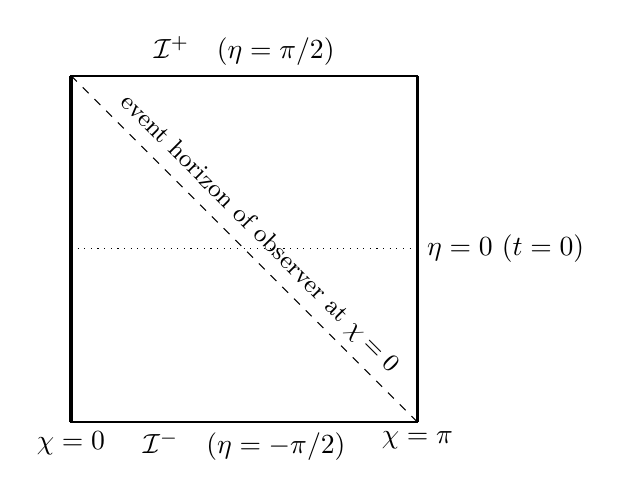
\begin{tikzpicture}[scale=1.1]
  % Square: horizontal axis chi in [0,pi] scaled to [0,4]; vertical axis eta in [-pi/2,pi/2] scaled to [0,4]
  \draw[thick] (0,0) rectangle (4,4);
  % Timelike worldlines chi=0 and chi=pi (poles of S^3)
  \draw[very thick] (0,0) -- (0,4);
  \draw[very thick] (4,0) -- (4,4);
  % t=0 slice (eta=0)
  \draw[dotted] (0,2) -- (4,2);
  % Event horizon of the observer at chi=0: null line from (chi,eta)=(0,pi/2) to (pi,-pi/2)
  \draw[dashed] (0,4) -- (4,0);
  % Labels
  \node[above] at (2,4) {$\mathcal I^+$\quad($\eta=\pi/2$)};
  \node[below] at (2,0) {$\mathcal I^-$\quad($\eta=-\pi/2$)};
  \node[below] at (0,0) {$\chi=0$};
  \node[below] at (4,0) {$\chi=\pi$};
  \node[right] at (4,2) {$\eta=0$ ($t=0$)};
  \node[rotate=-45, font=\small, above] at (2,2) {event horizon of observer at $\chi=0$};
\end{tikzpicture}
\end{center}

Diagram: square with horizontal coordinate $\chi\in(0,\pi)$ and vertical coordinate $\eta\in(-\pi/2,\pi/2)$. Each interior point represents a 2-sphere of radius $L\sin\chi/\cos\eta$, suppressed in the picture. The dashed diagonal is the causal horizon for the observer at $\chi=0$: it is the 45$^\circ$ null line through the endpoint of that observer's worldline on $\mathcal I^+$.

%---------------------------------------------------------------------------
\section*{Question 5 (6 points)}

\subsection*{(a) Gravitational waves from the linearised equation}

Choose the Lorenz (harmonic) gauge, $\partial^\mu\bar h_{\mu\nu}=0$. This is always achievable: under $h_{\mu\nu}\to h_{\mu\nu}+\partial_\mu\xi_\nu+\partial_\nu\xi_\mu$, the gauge condition changes by $\Box\xi_\nu$, which can be solved for $\xi$. In this gauge
\[
\partial^\rho\partial_{(\mu}\bar h_{\nu)\rho} = \tfrac12\partial_\mu(\partial^\rho\bar h_{\nu\rho}) + \tfrac12\partial_\nu(\partial^\rho\bar h_{\mu\rho}) = 0,
\qquad
\partial^\rho\partial^\sigma\bar h_{\rho\sigma}=0 .
\]
The linearised equation becomes
\[
-\tfrac12\Box\bar h_{\mu\nu} = 8\pi G\,T_{\mu\nu}
\quad\Longrightarrow\quad
\Box\bar h_{\mu\nu} = -16\pi G\,T_{\mu\nu}.
\]
In vacuum ($T_{\mu\nu}=0$) this is the wave equation $\left(-\partial_t^2+\nabla^2\right)\bar h_{\mu\nu}=0$. Its solutions propagate at the speed of light, so they are gravitational waves. The residual gauge freedom can further set $h=0$, $h_{0\mu}=0$ and $\partial^ih_{ij}=0$ (transverse-traceless gauge). Then $h_{ij}$ has only two independent polarisations, $+$ and $\times$.

\subsection*{(b) Proper distances between test particles}

For the metric $g_{\mu\nu}=\eta_{\mu\nu}+h_{\mu\nu}$ with only $h_{xx}=-h_{yy}=h_+(t-z)$ nonzero, the Christoffel symbols at linear order include
\[
\Gamma^i{}_{00} = \tfrac12\eta^{ij}\left(2\partial_0 h_{j0}-\partial_j h_{00}\right)=0,
\]
because $h_{00}=h_{0j}=0$. A freely falling particle starting at rest satisfies $\ddot x^i = -\Gamma^i{}_{00}+\mathcal O(h^2)=0$, so it stays at fixed coordinate position $x^i$. The proper distance at fixed $t$ is then measured by the spatial metric along the line joining the particles.

\textbf{Particles at $(0,0,0)$ and $(L_x,0,0)$.} Both lie in the plane $z=0$, so $h_+(t-z)=h_+(t)$ along the line, and it is independent of $x$. The proper length is
\[
\Delta s = \int_0^{L_x}\sqrt{g_{xx}}\,dx = \int_0^{L_x}\sqrt{1+h_+(t)}\,dx \approx \int_0^{L_x}\left(1+\tfrac12h_+(t)\right)dx = L_x\left(1+\tfrac12 h_+(t)\right).
\]

\textbf{Particle at $(0,L_y,0)$.} Here $g_{yy}=1+h_{yy}=1-h_+(t)$, so
\[
\Delta s = \int_0^{L_y}\sqrt{1-h_+(t)}\,dy \approx L_y\left(1-\tfrac12 h_+(t)\right).
\]
The wave stretches the $x$-separation and compresses the $y$-separation by the same fraction.

\subsection*{(c) Binary inspiral, merger and ringdown}

\textbf{Inspiral.} Two masses on a circular orbit radiate gravitational waves. The quadrupole power is $P=\frac{32}{5}\frac{G}{c^5}\mu^2r^4\omega^6$. The orbital energy is lost, so the separation $r$ shrinks. By Kepler's law $\omega^2=GM/r^3$, the orbital frequency rises as $r$ falls. The gravitational-wave frequency is twice the orbital frequency and increases, and the amplitude grows. This is the "chirp".

\textbf{Merger.} When the separation reaches a few times $GM/c^2$, the bodies plunge together. The emission is strongest here, the motion is highly non-linear, and a numerical-relativity calculation is needed. The signal reaches its peak amplitude.

\textbf{Ringdown.} The merged object is a perturbed black hole. It settles to a stationary Kerr black hole by emitting quasinormal modes. The signal becomes an exponentially damped sinusoid, with frequency and damping time set by the remnant's mass and spin.

\textbf{Detection by an interferometer.} Consider a Michelson interferometer with perpendicular arms of length $L$, along $x$ and $y$. A wave travelling along $z$ with $+$ polarisation, as in (b), changes the arm lengths to $L(1+\tfrac12h)$ and $L(1-\tfrac12h)$. The round-trip light times differ by
\[
\Delta\tau = \frac{2L}{c}\,h(t),
\]
so the beams recombine with phase difference $\Delta\phi = \omega\,\Delta\tau = \dfrac{4\pi L}{\lambda}\,h(t)$. The power at the output port changes in proportion to $h(t)$, so the detector measures the strain $h(t)$ directly. Real detectors use Fabry--Perot cavities to increase the effective arm length.

\textbf{Sketch of the signal.} The schematic below shows $h(t)$ as measured by the detector. It is not to scale.

\begin{center}
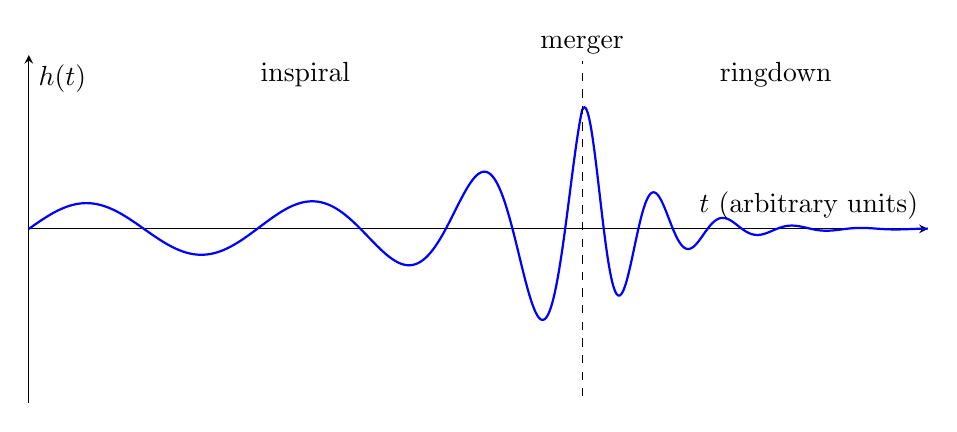
\begin{tikzpicture}
\begin{axis}[
  width=13cm, height=6cm,
  xmin=0, xmax=1.3, ymin=-1.35, ymax=1.35,
  axis lines=middle,
  xlabel={$t$ (arbitrary units)}, ylabel={$h(t)$},
  xtick=\empty, ytick=\empty,
  clip=false,
]
% Inspiral: amplitude and frequency both increase
\addplot[thick, blue, domain=0:0.8, samples=600]
  {(0.2+0.8*(x/0.8)^6)*sin(360*(3*x+2.4*x^5))};
% Ringdown: exponentially damped
\addplot[thick, blue, domain=0.8:1.3, samples=300]
  {exp(-12*(x-0.8))*sin(360*(3.1864+10*(x-0.8)))};
% Merger marker
\draw[dashed] (axis cs:0.8,-1.3) -- (axis cs:0.8,1.3);
\node at (axis cs:0.4,1.2) {inspiral};
\node at (axis cs:0.8,1.28) [anchor=south] {merger};
\node at (axis cs:1.08,1.2) {ringdown};
\end{axis}
\end{tikzpicture}
\end{center}

\textbf{Features of the signal.}
\begin{itemize}[leftmargin=2em]
\item The increasing frequency and amplitude during the inspiral reflect the shrinking orbit and the growing orbital frequency.
\item The peak corresponds to the merger, where the most gravitational-wave energy is emitted.
\item The exponentially damped tail corresponds to the remnant black hole ringing down to its final stationary state.
\end{itemize}

\end{document}
